% A simple Tree
% Author: Stefan Kottwitz
% https://www.packtpub.com/hardware-and-creative/latex-cookbook
\documentclass[border=0.2cm]{standalone}
\usepackage{tikz}
\usetikzlibrary{mindmap,backgrounds}
\usetikzlibrary{shapes.geometric,positioning}
\tikzset{
  treenode/.style = {shape=rectangle, rounded corners,
                     draw, align=center,
                     top color=white, bottom color=blue!20},
  root/.style     = {
    treenode,
    font=\fontfamily{ppl}\fontsize{2cm}{2cm}\selectfont,
    shape=rectangle, rounded corners, draw,
    align=center,
    top color=white,
    bottom color=cyan!60},
  centroid/.style      = {
    treenode,
    font=\huge\bfseries
    },
    instance/.style    = {
    circle, 
    draw,
    font=\ttfamily\Large
    }
}
\begin{document}



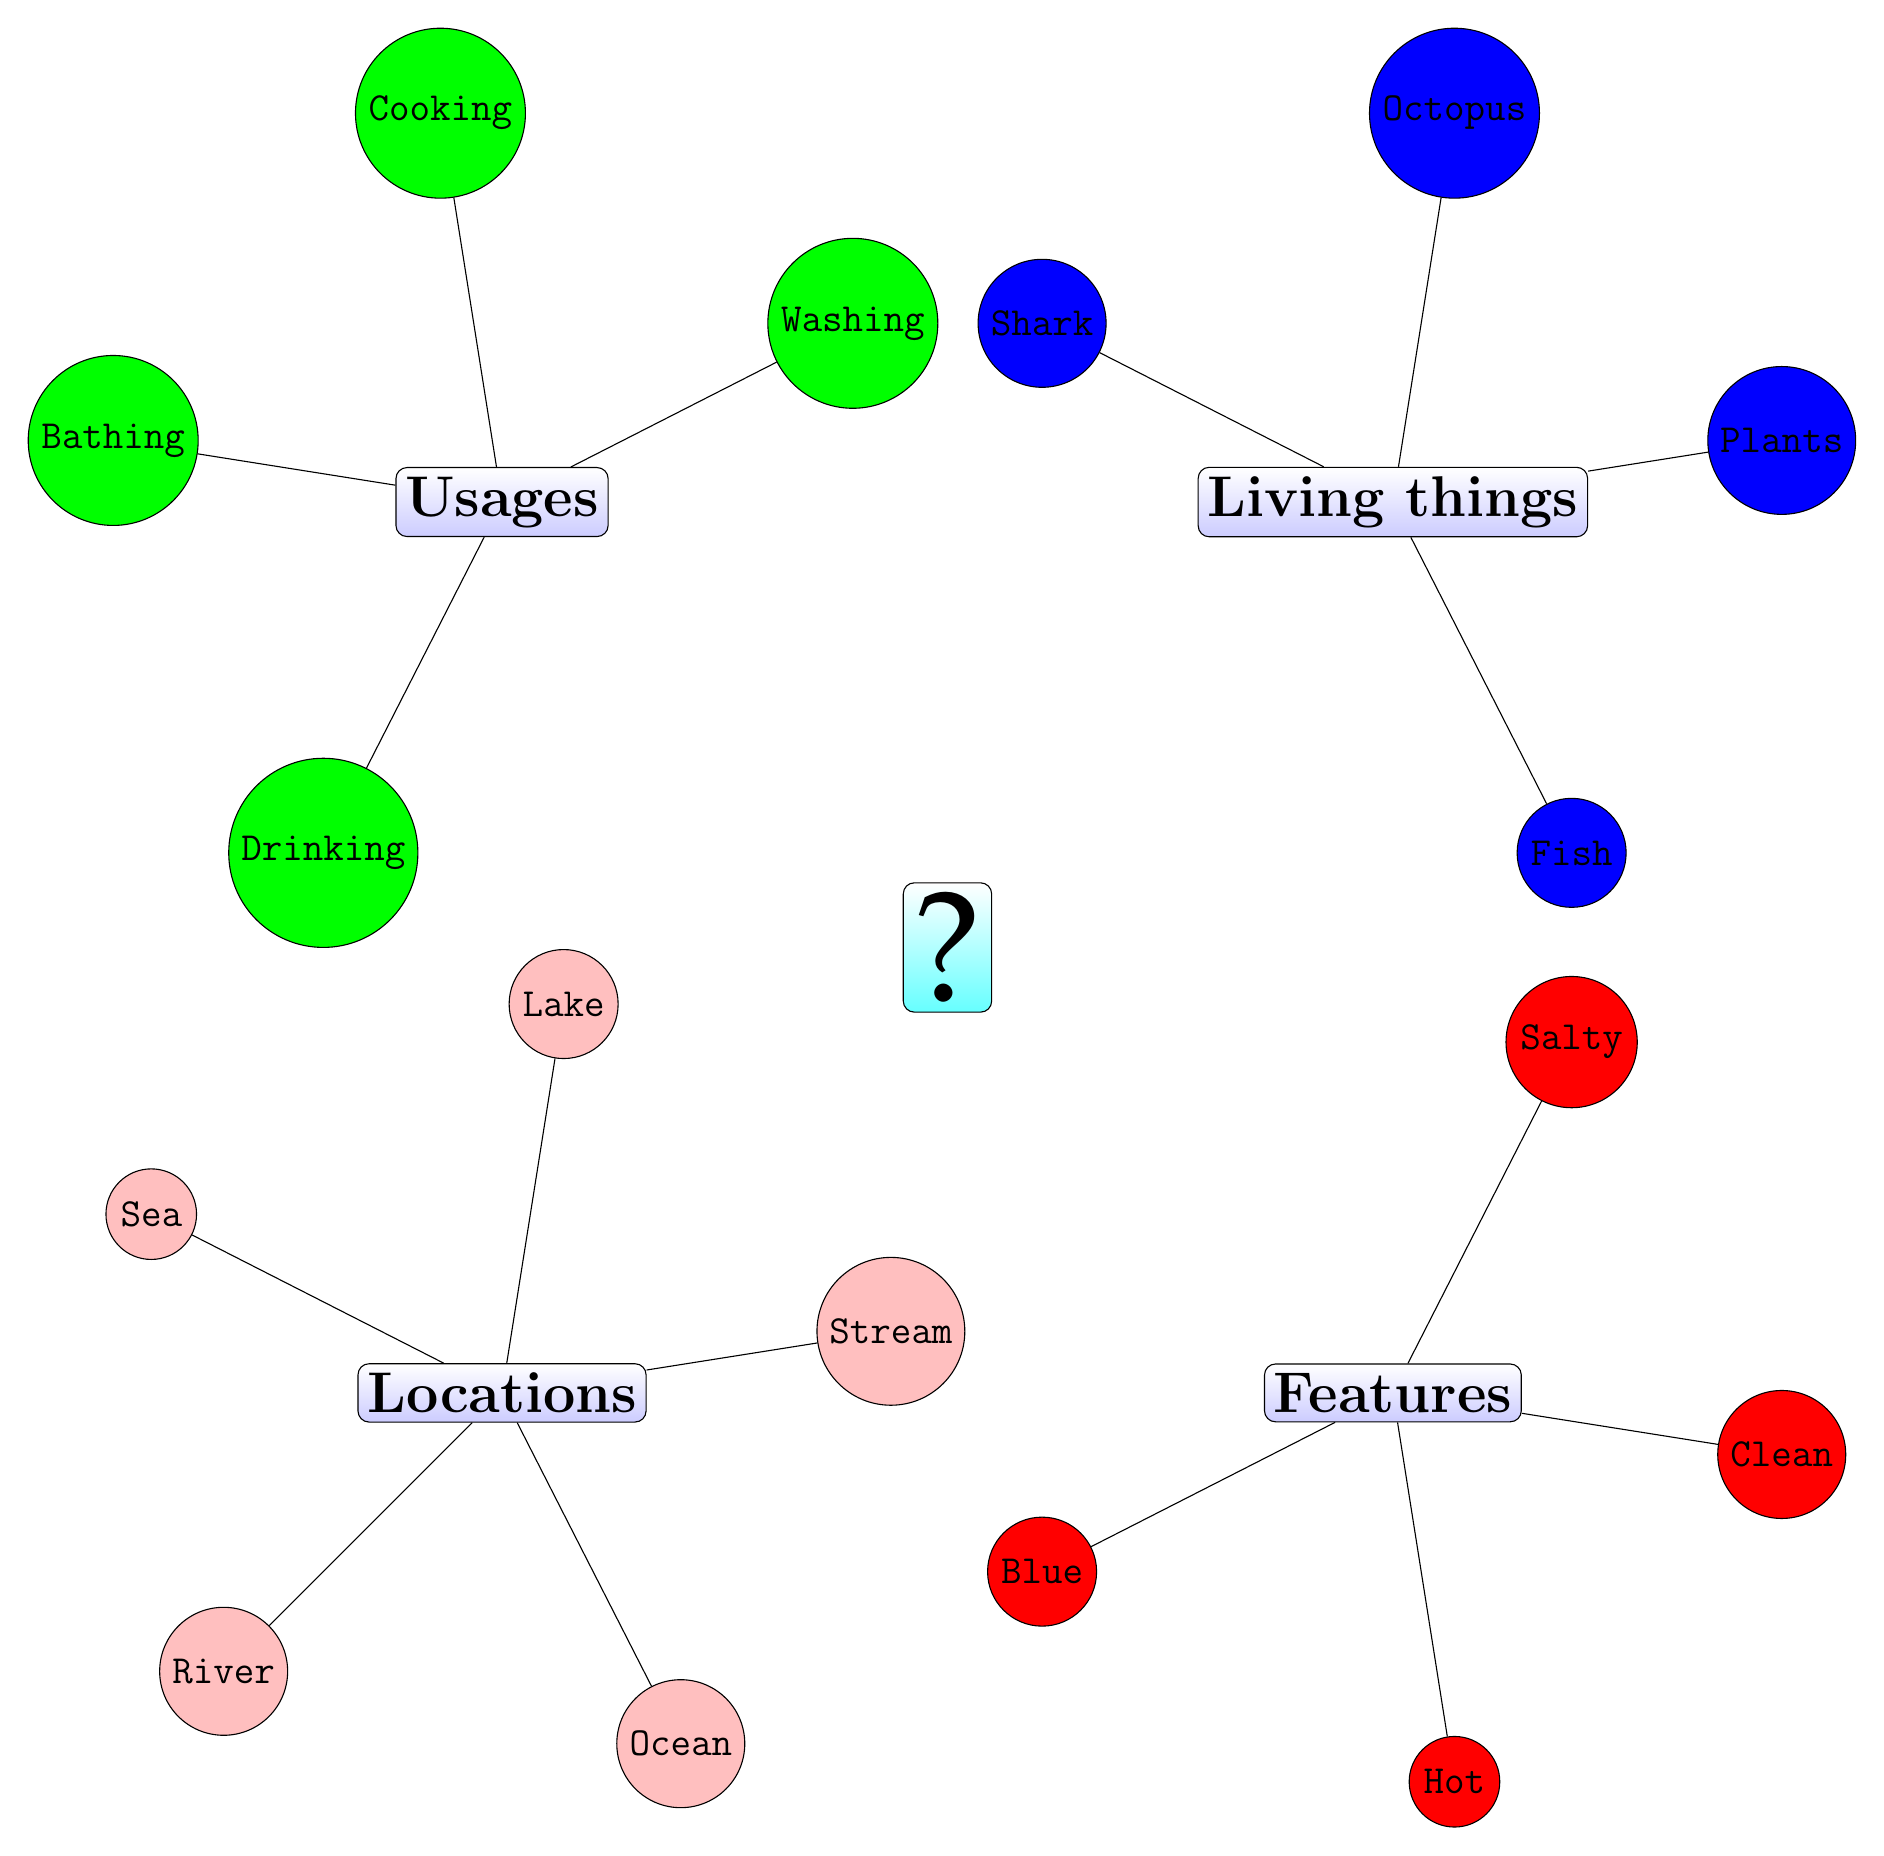
\begin{tikzpicture}[
    grow cyclic, 
    level 1/.style = {
        level distance = 8cm, 
        sibling angle = 90
        },
    level 2/.style = {
        level distance = 5cm, 
        sibling angle = 72
        }
    ]
    \node [root]{?}
        child {node [centroid] {Locations}
            child {node [instance, fill=pink] {Lake}}
            child {node [instance, fill=pink] {Sea}}
            child {node [instance, fill=pink] {River}}
            child {node [instance, fill=pink] {Ocean}}
            child {node [instance, fill=pink] {Stream}}
            edge from parent[draw=none]
            }
        child {node [centroid] {Features}
            child {node [instance, fill=red] {Blue}}
            child {node [instance, fill=red] {Hot}}
            child {node [instance, fill=red] {Clean}}
            child {node [instance, fill=red] {Salty}}
            edge from parent[draw=none]
            }
        child {node [centroid] {Living things}
            child {node [instance, fill=blue] {Fish}}
            child {node [instance, fill=blue] {Plants}}
            child {node [instance, fill=blue] {Octopus}}
            child {node [instance, fill=blue] {Shark}}
            edge from parent[draw=none]
            }
        child {node [centroid] {Usages}
            child {node [instance, fill=green] {Washing}}
            child {node [instance, fill=green] {Cooking}}
            child {node [instance, fill=green] {Bathing}}
            child {node [instance, fill=green] {Drinking}}
            edge from parent[draw=none]
            };
\end{tikzpicture}


\end{document}